\chapter{Puukyselyt}

Tyypillisiä puukyselyitä ovat
puun polkuihin ja alipuihin
liittyvät kyselyt.
Tämä luku esittelee
tekniikoita, joiden avulla on mahdollista
toteuttaa puukyselyjä tehokkaasti.
Usein esiintyvä idea on muuttaa
puu jollakin tavalla taulukoksi
ja hyödyntää tehokkaita taulukon välikyselyitä.

\section{Tehokas nouseminen}

\begin{task}
Annettuna on juurellinen puu, jonka solmut on numeroitu
$1 \ldots n$ ja juurisolmu on 1.
Tehtäväsi on vastata
tehokkaasti kyselyihin muotoa ''mikä solmu on
$k$ askelta ylempänä solmua $x$''.
\end{task}

Merkitään $f(x,k)$ solmua,
joka on $k$ askelta ylempänä solmua $x$.
Esimerkiksi seuraavassa puussa
$f(2,1)=1$ ja $f(8,2)=4$.

\begin{center}
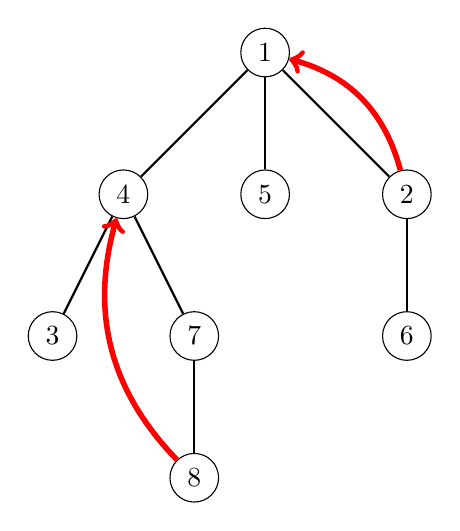
\begin{tikzpicture}[scale=0.9]
\node[draw, circle] (1) at (0,3) {$1$};
\node[draw, circle] (2) at (2,1) {$2$};
\node[draw, circle] (3) at (-2,1) {$4$};
\node[draw, circle] (4) at (0,1) {$5$};
\node[draw, circle] (5) at (2,-1) {$6$};
\node[draw, circle] (6) at (-3,-1) {$3$};
\node[draw, circle] (7) at (-1,-1) {$7$};
\node[draw, circle] (8) at (-1,-3) {$8$};
\path[draw,thick,-] (1) -- (2);
\path[draw,thick,-] (1) -- (3);
\path[draw,thick,-] (1) -- (4);
\path[draw,thick,-] (2) -- (5);
\path[draw,thick,-] (3) -- (6);
\path[draw,thick,-] (3) -- (7);
\path[draw,thick,-] (7) -- (8);

\path[draw=red,thick,->,line width=2pt] (8) edge [bend left] (3);
\path[draw=red,thick,->,line width=2pt] (2) edge [bend right] (1);
\end{tikzpicture}
\end{center}

Suoraviivainen tapa laskea funktion $f(x,k)$
arvo on kulkea puussa $k$ askelta ylöspäin
solmusta $x$ alkaen.
Tämän aikavaativuus on kuitenkin $O(n)$,
koska on mahdollista, että puussa on
ketju, jossa on $O(n)$ solmua.

Kuten luvussa 16.3.1, funktion $f(x,k)$
arvo on mahdollista laskea tehokkaasti ajassa
$O(\log k)$ sopivan esikäsittelyn avulla.
Ideana on laskea etukäteen kaikki arvot
$f(x,k)$, joissa $k=1,2,4,8,\ldots$ eli 2:n potenssi.
Esimerkiksi yllä olevassa puussa muodostuu seuraava taulukko:

\begin{center}
\begin{tabular}{r|rrrrrrrrr}
$x$ & 1 & 2 & 3 & 4 & 5 & 6 & 7 & 8 \\
\hline
$f(x,1)$ & 0 & 1 & 4 & 1 & 1 & 2 & 4 & 7 \\
$f(x,2)$ & 0 & 0 & 1 & 0 & 0 & 1 & 1 & 4 \\
$f(x,4)$ & 0 & 0 & 0 & 0 & 0 & 0 & 0 & 0 \\
$\cdots$ \\
\end{tabular}
\end{center}

Taulukossa arvo 0 tarkoittaa, että nousemalla $k$
askelta päätyy puun ulkopuolelle juurisolmun yläpuolelle.

Esilaskenta vie aikaa $O(n \log n)$, koska jokaisesta
solmusta voi nousta korkeintaan $n$ askelta ylöspäin.
Tämän jälkeen minkä tahansa funktion $f(x,k)$ arvon saa
laskettua ajassa $O(\log k)$ jakamalla nousun 2:n
potenssin osiin.

\section{Solmutaulukko}

Solmutaulukko sisältää juurellisen puun solmut siinä
järjestyksessä kuin juuresta alkava syvyyshaku
vierailee solmuissa.

Esimerkiksi puussa
\begin{center}
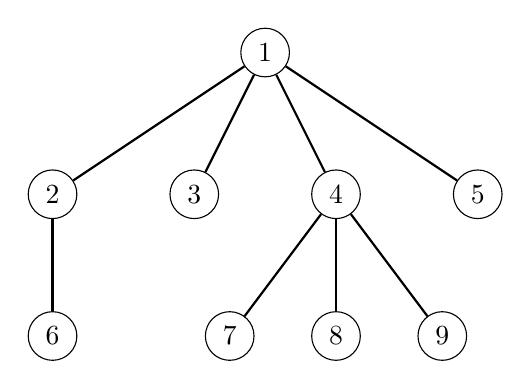
\begin{tikzpicture}[scale=0.9]
\node[draw, circle] (1) at (0,3) {$1$};
\node[draw, circle] (2) at (-3,1) {$2$};
\node[draw, circle] (3) at (-1,1) {$3$};
\node[draw, circle] (4) at (1,1) {$4$};
\node[draw, circle] (5) at (3,1) {$5$};
\node[draw, circle] (6) at (-3,-1) {$6$};
\node[draw, circle] (7) at (-0.5,-1) {$7$};
\node[draw, circle] (8) at (1,-1) {$8$};
\node[draw, circle] (9) at (2.5,-1) {$9$};

\path[draw,thick,-] (1) -- (2);
\path[draw,thick,-] (1) -- (3);
\path[draw,thick,-] (1) -- (4);
\path[draw,thick,-] (1) -- (5);
\path[draw,thick,-] (2) -- (6);
\path[draw,thick,-] (4) -- (7);
\path[draw,thick,-] (4) -- (8);
\path[draw,thick,-] (4) -- (9);
\end{tikzpicture}
\end{center}

syvyyshaku etenee

\begin{center}
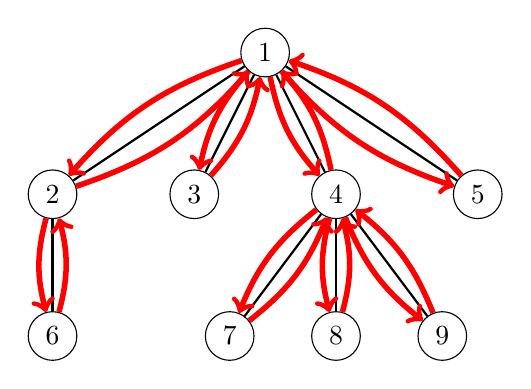
\begin{tikzpicture}[scale=0.9]
\node[draw, circle] (1) at (0,3) {$1$};
\node[draw, circle] (2) at (-3,1) {$2$};
\node[draw, circle] (3) at (-1,1) {$3$};
\node[draw, circle] (4) at (1,1) {$4$};
\node[draw, circle] (5) at (3,1) {$5$};
\node[draw, circle] (6) at (-3,-1) {$6$};
\node[draw, circle] (7) at (-0.5,-1) {$7$};
\node[draw, circle] (8) at (1,-1) {$8$};
\node[draw, circle] (9) at (2.5,-1) {$9$};

\path[draw,thick,-] (1) -- (2);
\path[draw,thick,-] (1) -- (3);
\path[draw,thick,-] (1) -- (4);
\path[draw,thick,-] (1) -- (5);
\path[draw,thick,-] (2) -- (6);
\path[draw,thick,-] (4) -- (7);
\path[draw,thick,-] (4) -- (8);
\path[draw,thick,-] (4) -- (9);


\path[draw=red,thick,->,line width=2pt] (1) edge [bend right=15] (2);
\path[draw=red,thick,->,line width=2pt] (2) edge [bend right=15] (6);
\path[draw=red,thick,->,line width=2pt] (6) edge [bend right=15] (2);
\path[draw=red,thick,->,line width=2pt] (2) edge [bend right=15] (1);
\path[draw=red,thick,->,line width=2pt] (1) edge [bend right=15] (3);
\path[draw=red,thick,->,line width=2pt] (3) edge [bend right=15] (1);
\path[draw=red,thick,->,line width=2pt] (1) edge [bend right=15] (4);
\path[draw=red,thick,->,line width=2pt] (4) edge [bend right=15] (7);
\path[draw=red,thick,->,line width=2pt] (7) edge [bend right=15] (4);
\path[draw=red,thick,->,line width=2pt] (4) edge [bend right=15] (8);
\path[draw=red,thick,->,line width=2pt] (8) edge [bend right=15] (4);
\path[draw=red,thick,->,line width=2pt] (4) edge [bend right=15] (9);
\path[draw=red,thick,->,line width=2pt] (9) edge [bend right=15] (4);
\path[draw=red,thick,->,line width=2pt] (4) edge [bend right=15] (1);
\path[draw=red,thick,->,line width=2pt] (1) edge [bend right=15] (5);
\path[draw=red,thick,->,line width=2pt] (5) edge [bend right=15] (1);

\end{tikzpicture}
\end{center}

ja solmutaulukoksi tulee:

\begin{center}
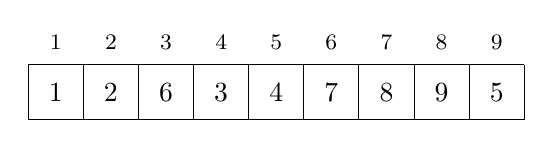
\begin{tikzpicture}[scale=0.7]
\draw (0,0) grid (9,1);

\node at (0.5,0.5) {$1$};
\node at (1.5,0.5) {$2$};
\node at (2.5,0.5) {$6$};
\node at (3.5,0.5) {$3$};
\node at (4.5,0.5) {$4$};
\node at (5.5,0.5) {$7$};
\node at (6.5,0.5) {$8$};
\node at (7.5,0.5) {$9$};
\node at (8.5,0.5) {$5$};

\footnotesize
\node at (0.5,1.4) {$1$};
\node at (1.5,1.4) {$2$};
\node at (2.5,1.4) {$3$};
\node at (3.5,1.4) {$4$};
\node at (4.5,1.4) {$5$};
\node at (5.5,1.4) {$6$};
\node at (6.5,1.4) {$7$};
\node at (7.5,1.4) {$8$};
\node at (8.5,1.4) {$9$};
\end{tikzpicture}
\end{center}

\subsection{Alipuiden käsittely}

Solmutaulukossa jokaisen alipuun kaikki solmut ovat peräkkäin
niin, että ensin on alipuun juurisolmu ja sitten
kaikki muut alipuun solmut.
Esimerkiksi äskeisessä taulukossa solmun $4$
alipuuta vastaa seuraava taulukon osa:

\begin{center}
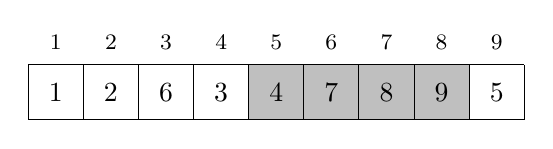
\begin{tikzpicture}[scale=0.7]
\fill[color=lightgray] (4,0) rectangle (8,1);
\draw (0,0) grid (9,1);

\node at (0.5,0.5) {$1$};
\node at (1.5,0.5) {$2$};
\node at (2.5,0.5) {$6$};
\node at (3.5,0.5) {$3$};
\node at (4.5,0.5) {$4$};
\node at (5.5,0.5) {$7$};
\node at (6.5,0.5) {$8$};
\node at (7.5,0.5) {$9$};
\node at (8.5,0.5) {$5$};

\footnotesize
\node at (0.5,1.4) {$1$};
\node at (1.5,1.4) {$2$};
\node at (2.5,1.4) {$3$};
\node at (3.5,1.4) {$4$};
\node at (4.5,1.4) {$5$};
\node at (5.5,1.4) {$6$};
\node at (6.5,1.4) {$7$};
\node at (7.5,1.4) {$8$};
\node at (8.5,1.4) {$9$};
\end{tikzpicture}
\end{center}

Tämän ansiosta solmutaulukon avulla voi käsitellä tehokkaasti
puun alipuihin liittyviä kyselyitä.
Voimme ratkaista esimerkiksi seuraavan tehtävän:

\begin{task}
Annettuna on juurellinen puu, jossa on $n$ solmua
ja jokaisella solmulla on tietty arvo.
Tehtäväsi on käsitellä kyselyt muotoa
''muuta solmun $x$ arvoa'' sekä
''laske arvojen summa solmun $x$ alipuussa''.
\end{task}

Tarkastellaan seuraavaa puuta,
jossa siniset luvut ovat solmujen arvoja.
Esimerkiksi solmun $4$ alipuun arvojen summa on $3+4+3+1=11$.

\begin{center}
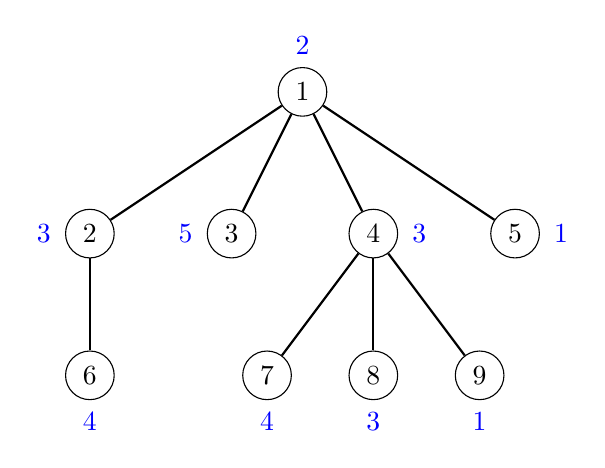
\begin{tikzpicture}[scale=0.9]
\node[draw, circle] (1) at (0,3) {$1$};
\node[draw, circle] (2) at (-3,1) {$2$};
\node[draw, circle] (3) at (-1,1) {$3$};
\node[draw, circle] (4) at (1,1) {$4$};
\node[draw, circle] (5) at (3,1) {$5$};
\node[draw, circle] (6) at (-3,-1) {$6$};
\node[draw, circle] (7) at (-0.5,-1) {$7$};
\node[draw, circle] (8) at (1,-1) {$8$};
\node[draw, circle] (9) at (2.5,-1) {$9$};

\path[draw,thick,-] (1) -- (2);
\path[draw,thick,-] (1) -- (3);
\path[draw,thick,-] (1) -- (4);
\path[draw,thick,-] (1) -- (5);
\path[draw,thick,-] (2) -- (6);
\path[draw,thick,-] (4) -- (7);
\path[draw,thick,-] (4) -- (8);
\path[draw,thick,-] (4) -- (9);

\node[color=blue] at (0,3+0.65) {2};
\node[color=blue] at (-3-0.65,1) {3};
\node[color=blue] at (-1-0.65,1) {5};
\node[color=blue] at (1+0.65,1) {3};
\node[color=blue] at (3+0.65,1) {1};
\node[color=blue] at (-3,-1-0.65) {4};
\node[color=blue] at (-0.5,-1-0.65) {4};
\node[color=blue] at (1,-1-0.65) {3};
\node[color=blue] at (2.5,-1-0.65) {1};
\end{tikzpicture}
\end{center}

Ideana on luoda solmutaulukko, joka sisältää jokaisesta solmusta
kolme tietoa: (1) solmun tunnus, (2) alipuun koko ja (3) solmun arvo.
Esimerkiksi yllä olevasta puusta syntyy seuraava taulukko:

\begin{center}
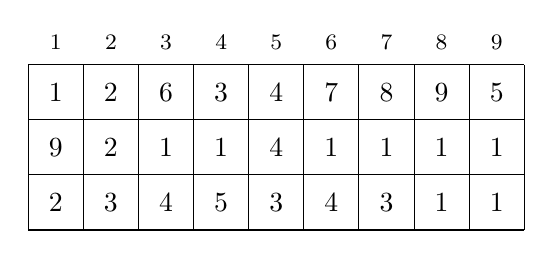
\begin{tikzpicture}[scale=0.7]
\draw (0,1) grid (9,-2);

\node at (0.5,0.5) {$1$};
\node at (1.5,0.5) {$2$};
\node at (2.5,0.5) {$6$};
\node at (3.5,0.5) {$3$};
\node at (4.5,0.5) {$4$};
\node at (5.5,0.5) {$7$};
\node at (6.5,0.5) {$8$};
\node at (7.5,0.5) {$9$};
\node at (8.5,0.5) {$5$};

\node at (0.5,-0.5) {$9$};
\node at (1.5,-0.5) {$2$};
\node at (2.5,-0.5) {$1$};
\node at (3.5,-0.5) {$1$};
\node at (4.5,-0.5) {$4$};
\node at (5.5,-0.5) {$1$};
\node at (6.5,-0.5) {$1$};
\node at (7.5,-0.5) {$1$};
\node at (8.5,-0.5) {$1$};

\node at (0.5,-1.5) {$2$};
\node at (1.5,-1.5) {$3$};
\node at (2.5,-1.5) {$4$};
\node at (3.5,-1.5) {$5$};
\node at (4.5,-1.5) {$3$};
\node at (5.5,-1.5) {$4$};
\node at (6.5,-1.5) {$3$};
\node at (7.5,-1.5) {$1$};
\node at (8.5,-1.5) {$1$};

\footnotesize
\node at (0.5,1.4) {$1$};
\node at (1.5,1.4) {$2$};
\node at (2.5,1.4) {$3$};
\node at (3.5,1.4) {$4$};
\node at (4.5,1.4) {$5$};
\node at (5.5,1.4) {$6$};
\node at (6.5,1.4) {$7$};
\node at (7.5,1.4) {$8$};
\node at (8.5,1.4) {$9$};
\end{tikzpicture}
\end{center}

Tästä taulukosta alipuun solmujen arvojen summa selviää
lukemalla ensin alipuun koko ja sitten sitä vastaavat solmut.
Esimerkiksi solmun $4$ alipuun arvojen summa selviää näin:

\begin{center}
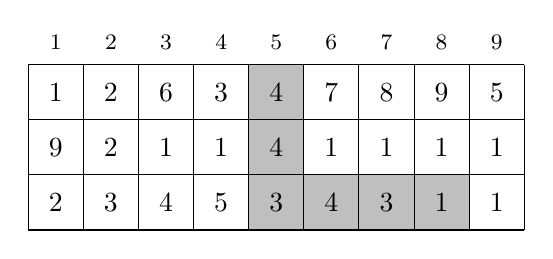
\begin{tikzpicture}[scale=0.7]
\fill[color=lightgray] (4,1) rectangle (5,0);
\fill[color=lightgray] (4,0) rectangle (5,-1);
\fill[color=lightgray] (4,-1) rectangle (8,-2);
\draw (0,1) grid (9,-2);

\node at (0.5,0.5) {$1$};
\node at (1.5,0.5) {$2$};
\node at (2.5,0.5) {$6$};
\node at (3.5,0.5) {$3$};
\node at (4.5,0.5) {$4$};
\node at (5.5,0.5) {$7$};
\node at (6.5,0.5) {$8$};
\node at (7.5,0.5) {$9$};
\node at (8.5,0.5) {$5$};

\node at (0.5,-0.5) {$9$};
\node at (1.5,-0.5) {$2$};
\node at (2.5,-0.5) {$1$};
\node at (3.5,-0.5) {$1$};
\node at (4.5,-0.5) {$4$};
\node at (5.5,-0.5) {$1$};
\node at (6.5,-0.5) {$1$};
\node at (7.5,-0.5) {$1$};
\node at (8.5,-0.5) {$1$};

\node at (0.5,-1.5) {$2$};
\node at (1.5,-1.5) {$3$};
\node at (2.5,-1.5) {$4$};
\node at (3.5,-1.5) {$5$};
\node at (4.5,-1.5) {$3$};
\node at (5.5,-1.5) {$4$};
\node at (6.5,-1.5) {$3$};
\node at (7.5,-1.5) {$1$};
\node at (8.5,-1.5) {$1$};

\footnotesize
\node at (0.5,1.4) {$1$};
\node at (1.5,1.4) {$2$};
\node at (2.5,1.4) {$3$};
\node at (3.5,1.4) {$4$};
\node at (4.5,1.4) {$5$};
\node at (5.5,1.4) {$6$};
\node at (6.5,1.4) {$7$};
\node at (7.5,1.4) {$8$};
\node at (8.5,1.4) {$9$};
\end{tikzpicture}
\end{center}

Viimeinen tarvittava askel on tallentaa solmujen arvot
binääri-indeksi\-puuhun tai segmenttipuuhun.
Tällöin sekä alipuun arvojen summan laskeminen
että solmun arvon muuttaminen onnistuvat ajassa $O(\log n)$,
eli pystymme vastaamaan kyselyihin tehokkaasti.

\subsection{Polkujen käsittely}

Solmutaulukon avulla voi myös käsitellä tehokkaasti
polkuja, jotka kulkevat juuresta tiettyyn solmuun puussa.
Näin on seuraavassa tehtävässä:

\begin{task}
Annettuna on juurellinen puu, jossa on $n$ solmua
ja jokaisella solmulla on tietty arvo.
Tehtäväsi on käsitellä kyselyt muotoa
''muuta solmun $x$ arvoa'' sekä
''laske arvojen summa juuresta solmuun $x$''.
\end{task}

Esimerkiksi seuraavassa puussa polulla solmusta 1
solmuun 8 arvojen summa on $4+5+3=12$.

\begin{center}
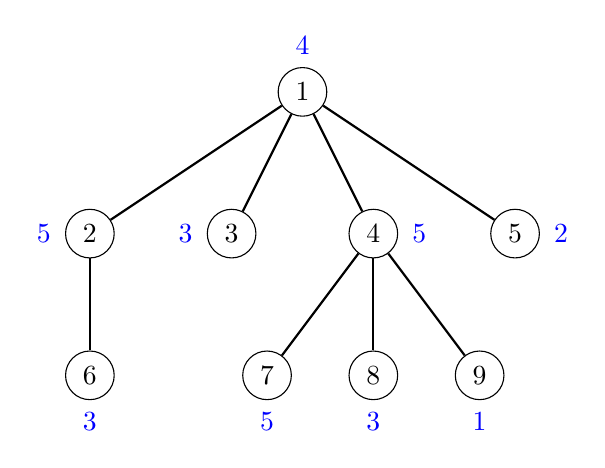
\begin{tikzpicture}[scale=0.9]
\node[draw, circle] (1) at (0,3) {$1$};
\node[draw, circle] (2) at (-3,1) {$2$};
\node[draw, circle] (3) at (-1,1) {$3$};
\node[draw, circle] (4) at (1,1) {$4$};
\node[draw, circle] (5) at (3,1) {$5$};
\node[draw, circle] (6) at (-3,-1) {$6$};
\node[draw, circle] (7) at (-0.5,-1) {$7$};
\node[draw, circle] (8) at (1,-1) {$8$};
\node[draw, circle] (9) at (2.5,-1) {$9$};

\path[draw,thick,-] (1) -- (2);
\path[draw,thick,-] (1) -- (3);
\path[draw,thick,-] (1) -- (4);
\path[draw,thick,-] (1) -- (5);
\path[draw,thick,-] (2) -- (6);
\path[draw,thick,-] (4) -- (7);
\path[draw,thick,-] (4) -- (8);
\path[draw,thick,-] (4) -- (9);

\node[color=blue] at (0,3+0.65) {4};
\node[color=blue] at (-3-0.65,1) {5};
\node[color=blue] at (-1-0.65,1) {3};
\node[color=blue] at (1+0.65,1) {5};
\node[color=blue] at (3+0.65,1) {2};
\node[color=blue] at (-3,-1-0.65) {3};
\node[color=blue] at (-0.5,-1-0.65) {5};
\node[color=blue] at (1,-1-0.65) {3};
\node[color=blue] at (2.5,-1-0.65) {1};
\end{tikzpicture}
\end{center}

Ideana on muodostaa samanlaiset taulukot kuin
alipuiden käsittelyssä mutta tallentaa
solmujen arvot erikoisella tavalla:
kun taulukon kohdassa $k$ olevan solmun arvo on $a$,
kohdan $k$ arvoon lisätään $a$ ja kohdan $k+c$ arvosta
vähennetään $a$, missä $c$ on alipuun koko.

Esimerkiksi yllä olevaa puuta vastaa seuraava taulukko:
\begin{center}
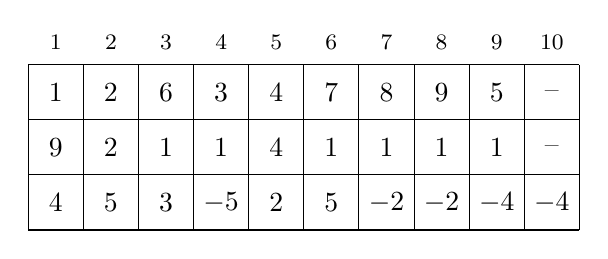
\begin{tikzpicture}[scale=0.7]
\draw (0,1) grid (10,-2);

\node at (0.5,0.5) {$1$};
\node at (1.5,0.5) {$2$};
\node at (2.5,0.5) {$6$};
\node at (3.5,0.5) {$3$};
\node at (4.5,0.5) {$4$};
\node at (5.5,0.5) {$7$};
\node at (6.5,0.5) {$8$};
\node at (7.5,0.5) {$9$};
\node at (8.5,0.5) {$5$};
\node at (9.5,0.5) {--};

\node at (0.5,-0.5) {$9$};
\node at (1.5,-0.5) {$2$};
\node at (2.5,-0.5) {$1$};
\node at (3.5,-0.5) {$1$};
\node at (4.5,-0.5) {$4$};
\node at (5.5,-0.5) {$1$};
\node at (6.5,-0.5) {$1$};
\node at (7.5,-0.5) {$1$};
\node at (8.5,-0.5) {$1$};
\node at (9.5,-0.5) {--};

\node at (0.5,-1.5) {$4$};
\node at (1.5,-1.5) {$5$};
\node at (2.5,-1.5) {$3$};
\node at (3.5,-1.5) {$-5$};
\node at (4.5,-1.5) {$2$};
\node at (5.5,-1.5) {$5$};
\node at (6.5,-1.5) {$-2$};
\node at (7.5,-1.5) {$-2$};
\node at (8.5,-1.5) {$-4$};
\node at (9.5,-1.5) {$-4$};

\footnotesize
\node at (0.5,1.4) {$1$};
\node at (1.5,1.4) {$2$};
\node at (2.5,1.4) {$3$};
\node at (3.5,1.4) {$4$};
\node at (4.5,1.4) {$5$};
\node at (5.5,1.4) {$6$};
\node at (6.5,1.4) {$7$};
\node at (7.5,1.4) {$8$};
\node at (8.5,1.4) {$9$};
\node at (9.5,1.4) {$10$};
\end{tikzpicture}
\end{center}

Esimerkiksi solmun $3$ arvona on $-5$, koska
se on solmujen $2$ ja $6$ alipuiden jälkeinen solmu,
mistä tulee arvoa $-5-3$, ja sen oma arvo on $3$.
Yhteensä solmun 3 arvo on siis $-5-3+3=-5$.
Huomaa, että taulukossa on ylimääräinen kohta 10,
johon on tallennettu vain juuren arvon vastaluku.

Nyt solmujen arvojen summa polulla juuresta alkaen
selviää laskemalla kaikkien taulukon arvojen summa
taulukon alusta solmuun asti.
Esimerkiksi summa solmusta $1$ solmuun $8$ selviää näin:

\begin{center}
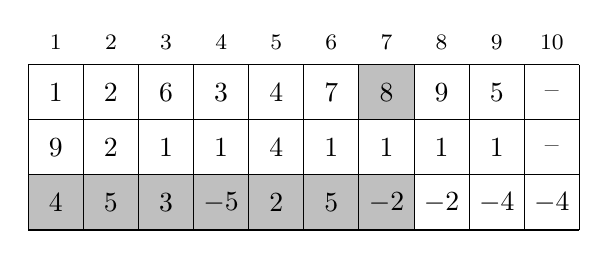
\begin{tikzpicture}[scale=0.7]
\fill[color=lightgray] (6,1) rectangle (7,0);
\fill[color=lightgray] (0,-1) rectangle (7,-2);
\draw (0,1) grid (10,-2);

\node at (0.5,0.5) {$1$};
\node at (1.5,0.5) {$2$};
\node at (2.5,0.5) {$6$};
\node at (3.5,0.5) {$3$};
\node at (4.5,0.5) {$4$};
\node at (5.5,0.5) {$7$};
\node at (6.5,0.5) {$8$};
\node at (7.5,0.5) {$9$};
\node at (8.5,0.5) {$5$};
\node at (9.5,0.5) {--};

\node at (0.5,-0.5) {$9$};
\node at (1.5,-0.5) {$2$};
\node at (2.5,-0.5) {$1$};
\node at (3.5,-0.5) {$1$};
\node at (4.5,-0.5) {$4$};
\node at (5.5,-0.5) {$1$};
\node at (6.5,-0.5) {$1$};
\node at (7.5,-0.5) {$1$};
\node at (8.5,-0.5) {$1$};
\node at (9.5,-0.5) {--};

\node at (0.5,-1.5) {$4$};
\node at (1.5,-1.5) {$5$};
\node at (2.5,-1.5) {$3$};
\node at (3.5,-1.5) {$-5$};
\node at (4.5,-1.5) {$2$};
\node at (5.5,-1.5) {$5$};
\node at (6.5,-1.5) {$-2$};
\node at (7.5,-1.5) {$-2$};
\node at (8.5,-1.5) {$-4$};
\node at (9.5,-1.5) {$-4$};

\footnotesize
\node at (0.5,1.4) {$1$};
\node at (1.5,1.4) {$2$};
\node at (2.5,1.4) {$3$};
\node at (3.5,1.4) {$4$};
\node at (4.5,1.4) {$5$};
\node at (5.5,1.4) {$6$};
\node at (6.5,1.4) {$7$};
\node at (7.5,1.4) {$8$};
\node at (8.5,1.4) {$9$};
\node at (9.5,1.4) {$10$};
\end{tikzpicture}
\end{center}

Summaksi tulee $4+5+3-5+2+5-2=12$, mikä vastaa
polun summaa $4+5+3=12$.
Tämä laskentatapa toimii, koska jokaisen solmun arvo
lisätään summaan, kun se tulee vastaan syvyyshaussa,
ja vähennetään summasta, kun sen käsittely päättyy.

Alipuiden käsittelyä vastaavasti voimme tallentaa
arvot binääri-indeksi\-puuhun tai segmenttipuuhun ja
sekä polun summan laskeminen että arvon muuttaminen
onnistuvat ajassa $O(\log n)$.

\section{Alin yhteinen esivanhempi}

Solmujen $a$ ja $b$
alin yhteinen esivanhempi (\textit{lowest common ancestor})
on mahdollisimman alhaalla puussa oleva solmu,
jonka alipuuhun kuuluvat molemmat solmut $a$ ja $b$.
Luonteva tehtävä on:

\begin{task}
Annettuna on puu, jossa on $n$ solmua.
Tehtäväsi on vastata kyselyihin
''mikä on solmujen $a$ ja $b$ alin yhteinen esivanhempi''.
\end{task}

\begin{samepage}
Esimerkiksi puussa

\begin{center}
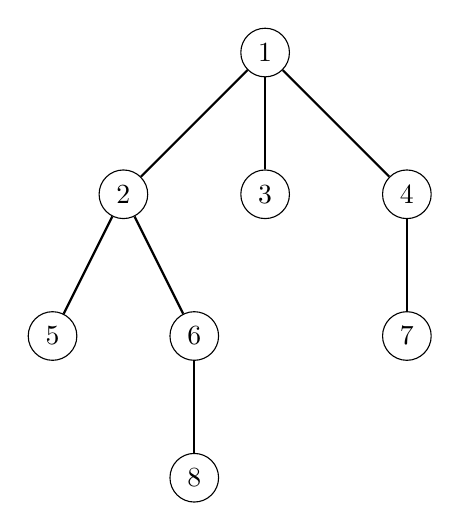
\begin{tikzpicture}[scale=0.9]
\node[draw, circle] (1) at (0,3) {$1$};
\node[draw, circle] (2) at (2,1) {$4$};
\node[draw, circle] (3) at (-2,1) {$2$};
\node[draw, circle] (4) at (0,1) {$3$};
\node[draw, circle] (5) at (2,-1) {$7$};
\node[draw, circle] (6) at (-3,-1) {$5$};
\node[draw, circle] (7) at (-1,-1) {$6$};
\node[draw, circle] (8) at (-1,-3) {$8$};
\path[draw,thick,-] (1) -- (2);
\path[draw,thick,-] (1) -- (3);
\path[draw,thick,-] (1) -- (4);
\path[draw,thick,-] (2) -- (5);
\path[draw,thick,-] (3) -- (6);
\path[draw,thick,-] (3) -- (7);
\path[draw,thick,-] (7) -- (8);
\end{tikzpicture}
\end{center}
\end{samepage}

solmujen 5 ja 8 alin yhteinen esivanhempi on solmu 2
ja solmujen 3 ja 4 alin yhteinen esivanhempi on solmu 1.

Tutustumme seuraavaksi kahteen menetelmään
alimman yhteisen esivanhemman selvittämiseen.

\subsubsection{Menetelmä 1}

Yksi tapa ratkaista tehtävä on hyödyntää
tehokasta nousemista puussa.
Tällöin alimman yhteisen esivanhemman etsiminen
muodostuu kahdesta vaiheesta.
Ensin noustaan alemmasta solmusta samalle tasolle
ylemmän solmun kanssa,
sitten noustaan rinnakkain kohti
alinta yhteistä esivanhempaa.

Tarkastellaan esimerkkinä solmujen 5 ja 8
alimman yhteisen esivanhemman etsimistä:

\begin{center}
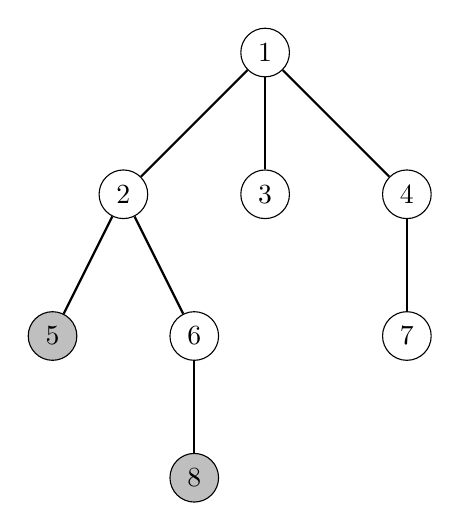
\begin{tikzpicture}[scale=0.9]
\node[draw, circle] (1) at (0,3) {$1$};
\node[draw, circle] (2) at (2,1) {$4$};
\node[draw, circle] (3) at (-2,1) {$2$};
\node[draw, circle] (4) at (0,1) {$3$};
\node[draw, circle] (5) at (2,-1) {$7$};
\node[draw, circle,fill=lightgray] (6) at (-3,-1) {$5$};
\node[draw, circle] (7) at (-1,-1) {$6$};
\node[draw, circle,fill=lightgray] (8) at (-1,-3) {$8$};
\path[draw,thick,-] (1) -- (2);
\path[draw,thick,-] (1) -- (3);
\path[draw,thick,-] (1) -- (4);
\path[draw,thick,-] (2) -- (5);
\path[draw,thick,-] (3) -- (6);
\path[draw,thick,-] (3) -- (7);
\path[draw,thick,-] (7) -- (8);
\end{tikzpicture}
\end{center}

Solmu 5 on tasolla 3, kun taas solmu 8 on tasolla 4.
Niinpä nousemme ensin solmusta 8 yhden tason ylemmäs solmuun 6:

\begin{center}
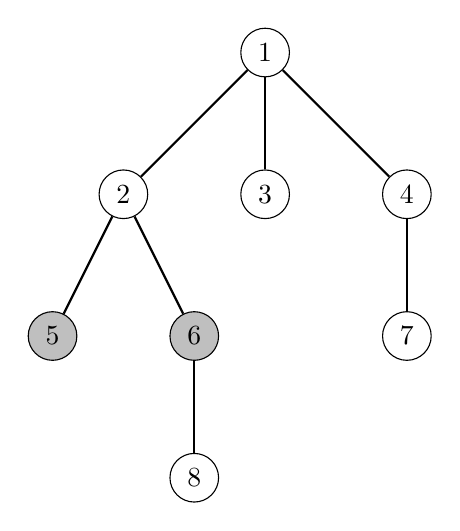
\begin{tikzpicture}[scale=0.9]
\node[draw, circle] (1) at (0,3) {$1$};
\node[draw, circle] (2) at (2,1) {$4$};
\node[draw, circle] (3) at (-2,1) {$2$};
\node[draw, circle] (4) at (0,1) {$3$};
\node[draw, circle] (5) at (2,-1) {$7$};
\node[draw, circle,fill=lightgray] (6) at (-3,-1) {$5$};
\node[draw, circle,fill=lightgray] (7) at (-1,-1) {$6$};
\node[draw, circle] (8) at (-1,-3) {$8$};
\path[draw,thick,-] (1) -- (2);
\path[draw,thick,-] (1) -- (3);
\path[draw,thick,-] (1) -- (4);
\path[draw,thick,-] (2) -- (5);
\path[draw,thick,-] (3) -- (6);
\path[draw,thick,-] (3) -- (7);
\path[draw,thick,-] (7) -- (8);
\end{tikzpicture}
\end{center}

Tämän jälkeen etsitään pienin määrä tasoja,
jotka nousemalla ylöspäin päädymme samaan solmuun.
Tässä tapauksessa riittää nousta yksi taso ylöspäin
solmuun 2. Niinpä solmujen alin yhteinen esivanhempi on 2:

\begin{center}
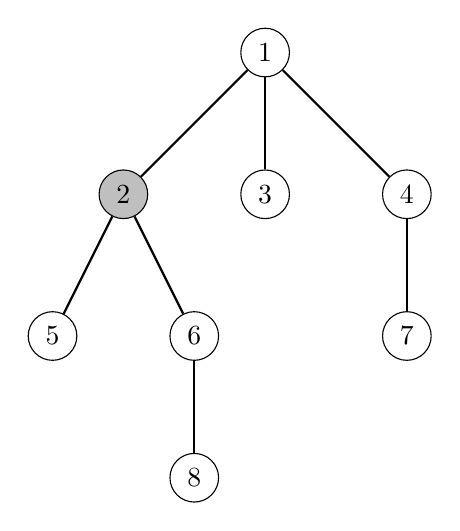
\begin{tikzpicture}[scale=0.9]
\node[draw, circle] (1) at (0,3) {$1$};
\node[draw, circle] (2) at (2,1) {$4$};
\node[draw, circle,fill=lightgray] (3) at (-2,1) {$2$};
\node[draw, circle] (4) at (0,1) {$3$};
\node[draw, circle] (5) at (2,-1) {$7$};
\node[draw, circle] (6) at (-3,-1) {$5$};
\node[draw, circle] (7) at (-1,-1) {$6$};
\node[draw, circle] (8) at (-1,-3) {$8$};
\path[draw,thick,-] (1) -- (2);
\path[draw,thick,-] (1) -- (3);
\path[draw,thick,-] (1) -- (4);
\path[draw,thick,-] (2) -- (5);
\path[draw,thick,-] (3) -- (6);
\path[draw,thick,-] (3) -- (7);
\path[draw,thick,-] (7) -- (8);
\end{tikzpicture}
\end{center}

Menetelmä vaatii $O(n \log n)$-aikaisen esikäsittelyn,
jonka jälkeen minkä tahansa kahden solmun alin yhteinen
esivanhempi selviää ajassa $O(\log n)$,
koska kumpikin vaihe nousussa vie aikaa $O(\log n)$.

\subsubsection{Menetelmä 2}

Toinen tapa ratkaista tehtävä perustuu solmutaulukon
käyttämiseen.
Ideana on jälleen järjestää solmut syvyyshaun mukaan:

\begin{center}
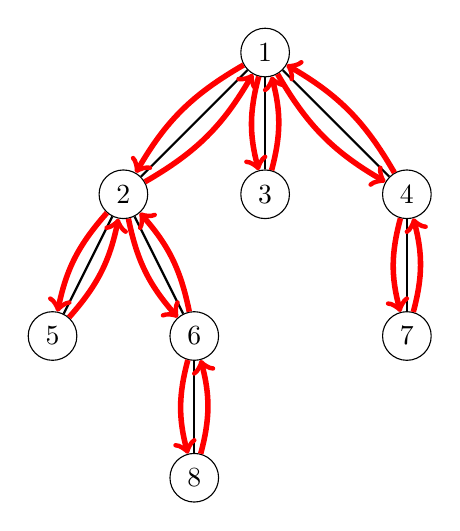
\begin{tikzpicture}[scale=0.9]
\node[draw, circle] (1) at (0,3) {$1$};
\node[draw, circle] (2) at (2,1) {$4$};
\node[draw, circle] (3) at (-2,1) {$2$};
\node[draw, circle] (4) at (0,1) {$3$};
\node[draw, circle] (5) at (2,-1) {$7$};
\node[draw, circle] (6) at (-3,-1) {$5$};
\node[draw, circle] (7) at (-1,-1) {$6$};
\node[draw, circle] (8) at (-1,-3) {$8$};
\path[draw,thick,-] (1) -- (2);
\path[draw,thick,-] (1) -- (3);
\path[draw,thick,-] (1) -- (4);
\path[draw,thick,-] (2) -- (5);
\path[draw,thick,-] (3) -- (6);
\path[draw,thick,-] (3) -- (7);
\path[draw,thick,-] (7) -- (8);

\path[draw=red,thick,->,line width=2pt] (1) edge [bend right=15] (3);
\path[draw=red,thick,->,line width=2pt] (3) edge [bend right=15] (6);
\path[draw=red,thick,->,line width=2pt] (6) edge [bend right=15] (3);
\path[draw=red,thick,->,line width=2pt] (3) edge [bend right=15] (7);
\path[draw=red,thick,->,line width=2pt] (7) edge [bend right=15] (8);
\path[draw=red,thick,->,line width=2pt] (8) edge [bend right=15] (7);
\path[draw=red,thick,->,line width=2pt] (7) edge [bend right=15] (3);
\path[draw=red,thick,->,line width=2pt] (3) edge [bend right=15] (1);
\path[draw=red,thick,->,line width=2pt] (1) edge [bend right=15] (4);
\path[draw=red,thick,->,line width=2pt] (4) edge [bend right=15] (1);
\path[draw=red,thick,->,line width=2pt] (1) edge [bend right=15] (2);
\path[draw=red,thick,->,line width=2pt] (2) edge [bend right=15] (5);
\path[draw=red,thick,->,line width=2pt] (5) edge [bend right=15] (2);
\path[draw=red,thick,->,line width=2pt] (2) edge [bend right=15] (1);
\end{tikzpicture}
\end{center}

Erona aiempaan solmu lisätään kuitenkin solmutaulukkoon
mukaan \textit{aina}, kun syvyyshaku käy solmussa,
eikä vain ensimmäisellä kerralla.
Niinpä solmu esiintyy solmutaulukossa $x+1$ kertaa,
missä $x$ on solmun lasten määrä,
ja solmutaulukossa on yhteensä $2n-1$ solmua.

Tallennamme solmutaulukkoon kaksi tietoa:
(1) solmun tunnus ja (2) solmun taso puussa.
Esimerkkipuuta vastaavat taulukot ovat:

\begin{center}
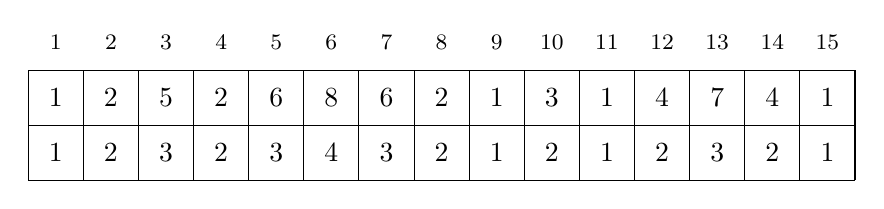
\begin{tikzpicture}[scale=0.7]

\draw (0,1) grid (15,2);
%\node at (-1.1,1.5) {\texttt{node}};
\node at (0.5,1.5) {$1$};
\node at (1.5,1.5) {$2$};
\node at (2.5,1.5) {$5$};
\node at (3.5,1.5) {$2$};
\node at (4.5,1.5) {$6$};
\node at (5.5,1.5) {$8$};
\node at (6.5,1.5) {$6$};
\node at (7.5,1.5) {$2$};
\node at (8.5,1.5) {$1$};
\node at (9.5,1.5) {$3$};
\node at (10.5,1.5) {$1$};
\node at (11.5,1.5) {$4$};
\node at (12.5,1.5) {$7$};
\node at (13.5,1.5) {$4$};
\node at (14.5,1.5) {$1$};


\draw (0,0) grid (15,1);
%\node at (-1.1,0.5) {\texttt{depth}};
\node at (0.5,0.5) {$1$};
\node at (1.5,0.5) {$2$};
\node at (2.5,0.5) {$3$};
\node at (3.5,0.5) {$2$};
\node at (4.5,0.5) {$3$};
\node at (5.5,0.5) {$4$};
\node at (6.5,0.5) {$3$};
\node at (7.5,0.5) {$2$};
\node at (8.5,0.5) {$1$};
\node at (9.5,0.5) {$2$};
\node at (10.5,0.5) {$1$};
\node at (11.5,0.5) {$2$};
\node at (12.5,0.5) {$3$};
\node at (13.5,0.5) {$2$};
\node at (14.5,0.5) {$1$};

\footnotesize
\node at (0.5,2.5) {$1$};
\node at (1.5,2.5) {$2$};
\node at (2.5,2.5) {$3$};
\node at (3.5,2.5) {$4$};
\node at (4.5,2.5) {$5$};
\node at (5.5,2.5) {$6$};
\node at (6.5,2.5) {$7$};
\node at (7.5,2.5) {$8$};
\node at (8.5,2.5) {$9$};
\node at (9.5,2.5) {$10$};
\node at (10.5,2.5) {$11$};
\node at (11.5,2.5) {$12$};
\node at (12.5,2.5) {$13$};
\node at (13.5,2.5) {$14$};
\node at (14.5,2.5) {$15$};
\end{tikzpicture}
\end{center}

Tämän taulukon avulla solmujen $a$ ja $b$ alin yhteinen esivanhempi
selviää etsimällä taulukosta alimman tason solmu
solmujen $a$ ja $b$ välissä.
Esimerkiksi solmujen 5 ja 8 alin yhteinen esivanhempi
löytyy seuraavasti:

\begin{center}
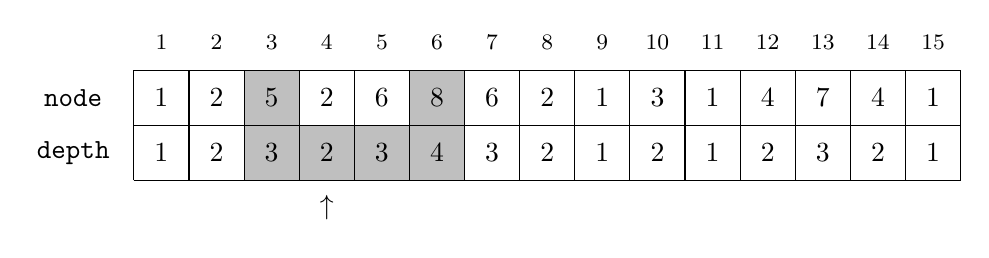
\begin{tikzpicture}[scale=0.7]
\fill[color=lightgray] (2,1) rectangle (3,2);
\fill[color=lightgray] (5,1) rectangle (6,2);
\fill[color=lightgray] (2,0) rectangle (6,1);

\node at (3.5,-0.5) {$\uparrow$};

\draw (0,1) grid (15,2);
\node at (-1.1,1.5) {\texttt{node}};
\node at (0.5,1.5) {$1$};
\node at (1.5,1.5) {$2$};
\node at (2.5,1.5) {$5$};
\node at (3.5,1.5) {$2$};
\node at (4.5,1.5) {$6$};
\node at (5.5,1.5) {$8$};
\node at (6.5,1.5) {$6$};
\node at (7.5,1.5) {$2$};
\node at (8.5,1.5) {$1$};
\node at (9.5,1.5) {$3$};
\node at (10.5,1.5) {$1$};
\node at (11.5,1.5) {$4$};
\node at (12.5,1.5) {$7$};
\node at (13.5,1.5) {$4$};
\node at (14.5,1.5) {$1$};


\draw (0,0) grid (15,1);
\node at (-1.1,0.5) {\texttt{depth}};
\node at (0.5,0.5) {$1$};
\node at (1.5,0.5) {$2$};
\node at (2.5,0.5) {$3$};
\node at (3.5,0.5) {$2$};
\node at (4.5,0.5) {$3$};
\node at (5.5,0.5) {$4$};
\node at (6.5,0.5) {$3$};
\node at (7.5,0.5) {$2$};
\node at (8.5,0.5) {$1$};
\node at (9.5,0.5) {$2$};
\node at (10.5,0.5) {$1$};
\node at (11.5,0.5) {$2$};
\node at (12.5,0.5) {$3$};
\node at (13.5,0.5) {$2$};
\node at (14.5,0.5) {$1$};

\footnotesize
\node at (0.5,2.5) {$1$};
\node at (1.5,2.5) {$2$};
\node at (2.5,2.5) {$3$};
\node at (3.5,2.5) {$4$};
\node at (4.5,2.5) {$5$};
\node at (5.5,2.5) {$6$};
\node at (6.5,2.5) {$7$};
\node at (7.5,2.5) {$8$};
\node at (8.5,2.5) {$9$};
\node at (9.5,2.5) {$10$};
\node at (10.5,2.5) {$11$};
\node at (11.5,2.5) {$12$};
\node at (12.5,2.5) {$13$};
\node at (13.5,2.5) {$14$};
\node at (14.5,2.5) {$15$};
\end{tikzpicture}
\end{center}

Solmu 5 on taulukossa kohdassa 3,
solmu 8 on taulukossa kohdassa 6
ja alimman tason solmu välillä $3 \ldots 6$
on kohdassa 4 oleva solmu 2,
jonka taso on 2.
Niinpä solmujen 5 ja 8 alin yhteinen esivanhempi
on solmu 2.

Alimman tason solmu välillä selviää
ajassa $O(\log n)$, kun taulukon sisältö on
tallennettu segmenttipuuhun.
Myös aikavaativuus $O(1)$ on mahdollinen,
koska taulukko on staattinen, mutta tälle on harvoin tarvetta.
Kummassakin tapauksessa esikäsittely vie aikaa $O(n \log n)$.

\subsubsection{Solmujen etäisyydet}

Myös seuraava tehtävä palautuu alimman yhteisen
esivanhemman hakuun:
\begin{task}
Annettuna on juurellinen puu, jonka solmut on numeroitu $1 \ldots n$.
Tehtäväsi on vastata kyselyihin
''laske solmujen $a$ ja $b$ etäisyys puussa''.
\end{task}

Valitaan ensin mikä tahansa
solmu puun juureksi.
Tämän jälkeen solmujen $a$ ja $b$
etäisyys on $d(a)+d(b)-2 \cdot d(c)$,
missä $c$ on solmujen alin yhteinen esivanhempi
ja $d(s)$ on etäisyys puun juuresta solmuun $s$.
Esimerkiksi puussa

\begin{center}
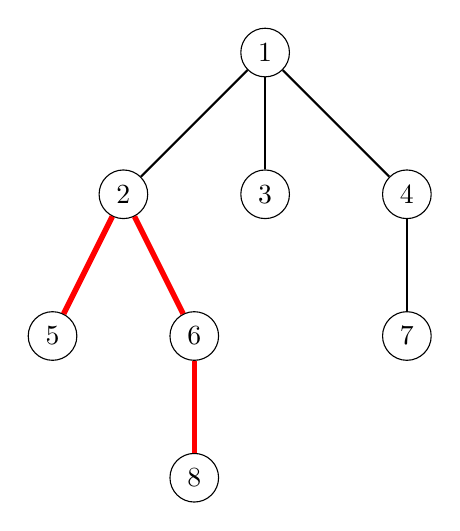
\begin{tikzpicture}[scale=0.9]
\node[draw, circle] (1) at (0,3) {$1$};
\node[draw, circle] (2) at (2,1) {$4$};
\node[draw, circle] (3) at (-2,1) {$2$};
\node[draw, circle] (4) at (0,1) {$3$};
\node[draw, circle] (5) at (2,-1) {$7$};
\node[draw, circle] (6) at (-3,-1) {$5$};
\node[draw, circle] (7) at (-1,-1) {$6$};
\node[draw, circle] (8) at (-1,-3) {$8$};
\path[draw,thick,-] (1) -- (2);
\path[draw,thick,-] (1) -- (3);
\path[draw,thick,-] (1) -- (4);
\path[draw,thick,-] (2) -- (5);
\path[draw,thick,-] (3) -- (6);
\path[draw,thick,-] (3) -- (7);
\path[draw,thick,-] (7) -- (8);

\path[draw=red,thick,-,line width=2pt] (8) -- node[font=\small] {} (7);
\path[draw=red,thick,-,line width=2pt] (7) -- node[font=\small] {} (3);
\path[draw=red,thick,-,line width=2pt] (6) -- node[font=\small] {} (3);
\end{tikzpicture}
\end{center}

solmujen 5 ja 8 alin yhteinen esivanhempi on 2.
Polku solmusta 5 solmuun 8
kulkee ensin ylöspäin solmusta 5
solmuun 2 ja sitten alaspäin
solmusta 2 solmuun 8.
Solmujen etäisyydet juuresta ovat $d(5)=3$,
$d(8)=4$ ja $d(2)=2$,
joten solmujen 5 ja 8 etäisyys
on $3+4-2\cdot2=3$.
